\documentclass{beamer}

% Import fonts and language packages
\usepackage{fontspec}
\usepackage[english]{babel}
\usepackage{algpseudocode}
\usepackage{amsthm} % for theorems
\usepackage{amsmath} % for \text and align environments
\usepackage{tikz}
\usepackage{xcolor}
\usepackage{caption}
\usepackage{subcaption}
\usetikzlibrary{backgrounds}
\usetikzlibrary{positioning}

% Use serif font
\usefonttheme{serif}

% Set the font to Times New Roman
\setmainfont{Times New Roman}

% Use Boadilla theme
\usetheme{Boadilla}

% Define dark blue color
\definecolor{darkblue}{RGB}{0,0,153}

% Set document information
\title[Email: 23B954005@stu.hit.edu.cn]{\textbf{HITsz Beamer Presentation}}
\author[{Presenter:  Chen}]{\fontsize{8}{10}\selectfont Presenter: Chen \\[10pt] Advisor: Professor  Chen}
\institute[HITsz]{\fontsize{8}{10}\selectfont School of Civil and Environmental Engineering \\ Harbin Institute of Technology, Shenzhen}
\date[\today]{\fontsize{8}{10}\selectfont \today}

% Customize frame title format
\setbeamertemplate{frametitle}[default][center]
\setbeamerfont{frametitle}{series=\bfseries}

% Begin document
\begin{document}
    \logo{}
    \begin{frame}
        \titlepage
        \begin{center}
            \vspace{-20pt}
            
\includegraphics[width=0.3\linewidth]{hitsz.pdf}
        \end{center}
    \end{frame}

% Create table of contents
    \logo{}
    \begin{frame}
        \frametitle{Contents}
        \tableofcontents
    \end{frame}
    \logo{}

% Section: Introduction
\section{Introduction}

% Display table of contents at the beginning of each section
\frame{\frametitle{Outline}\tableofcontents[currentsection]}
\subsection{Introduction}
\begin{frame}{Introduction}
  \begin{itemize}
    \item  The main purpose is to illustrate how to use Beamer syntax to organize content and to demonstrate some basic syntax for future reference.
    \item  We share an open-source LaTeX implementation of this template at \href{https://github.com/Chen861368/HITsz-Academic-Beamer-Template}{https://github.com/Chen861368/HITsz-Academic-Beamer-Template}.
\end{itemize}
 
  \vspace{10pt}

  \begin{table}[ht]
    \centering
    \begin{tabular}{|c|c|c|}
      \hline
      \textbf{Header 1} & \textbf{Header 2} & \textbf{Header 3} \\
      \hline
      Row 1, Col 1 & Row 1, Col 2 & Row 1, Col 3 \\
      \hline
      Row 2, Col 1 & Row 2, Col 2 & Row 2, Col 3 \\
      \hline
      Row 3, Col 1 & Row 3, Col 2 & Row 3, Col 3 \\
      \hline
    \end{tabular}
  \end{table}

\end{frame}

\subsection{Document Overview}
\begin{frame}{Document Overview}
  \begin{itemize}
      \item \textbf{Introduction:} Overview of the research problem and objectives.
      \item \textbf{Mathematical Estimation Problem:} Detailed explanation of the estimation problem and its formulation.
      \item \textbf{Kalman Filter:} Introduction to the Kalman filter and its application in state estimation.
      \item \textbf{Numerical Example:} Demonstration of the methodology using a Multi-Degree-Of-Freedom (MDOF) system.
      \item \textbf{Hamilton's Principle:} Explanation of the principle and its role in deriving equations of motion.
      \item \textbf{Conclusion:} Summary of findings and future work.
  \end{itemize}
\end{frame}

% Section: Main Content
\section{Main Content}

% Display table of contents at the beginning of each section
\frame{\frametitle{Outline}\tableofcontents[currentsection]}

% Subsection: The Mathematical Estimation problem
\subsection{The Mathematical Estimation problem}

\begin{frame}{The Mathematical Estimation problem}

  {\textcolor{red}{\textbf{The estimation problem}}} is mathematically formulated as determining parameters \(\theta\) from a discrete dataset \(\{x_0, x_1, ..., x_N\}\),
  associated with a signal following a stochastic model \( x \sim f(x, \theta) \)\cite{luLearningNonlinearOperators2021a,majumdarAutoencoderBasedFormulation2018}. 

  \vspace{10pt}

   \begin{itemize}
    \item The Mathematical Estimation Problem encompasses the challenge of inferring unknown parameters or system states from observational data. 
    \item Digital computers allow us to analyze sampled data, leading to the problem of estimating parameters from a discrete dataset.
    \item Parameter \(\theta\) is deterministic in classical and random in Bayesian estimation.
  \end{itemize}


   \vspace{10pt}

   The aim is to find \(\theta\) or construct an estimator \(\hat{\theta}\) using the function \( g \), expressed as:
  \[
  \hat{\theta} = g(x_0, x_1, ..., x_N)
  \]
  
  Here, the function \( g \) is designed to estimate the parameters \(\theta\) from the data.
\end{frame}

\begin{frame}{The Mathematical Estimation problem}
Often, the main trick is finding the right mathematical formulation of your estimation problem 
\begin{itemize}
  \item \textbf{Function \( x \sim f(x, \theta) \)}: Identify the function that best represents the data or the system.
  \item \textbf{Metric \( L(\theta, \hat{\theta}) \)}: Choose a loss or cost function \( L \) that quantifies the error or difference between the estimated parameters \( \hat{\theta} \) and the true parameters \( \theta \).
  \item \textbf{Constraints \( R(\theta) \)}: Define any constraints \( R \) that the parameters \( \theta \) must satisfy. These could be physical constraints, regulatory requirements, or computational limitations.
\end{itemize}

\begin{block}{Algorithm Selection}
  \begin{itemize}
      \item Once the function, metric, and  constraints are defined, the next step is to choose the best algorithms that 
      exploit these definitions to solve the estimation problem effectively.
  \end{itemize}
\end{block}

\end{frame}



\begin{frame}{Kalman Filter}
  \begin{itemize}
          \item State Space (White box)
          \item Prediction-Correction (Recursion)
  \end{itemize}
  The Kalman filter model assumes the true state at time $n+1$ is evolved from the state at $n$ according to
  \begin{align*}
    x_{n+1} &= A_n x_n + v_n \\
    y_n &= C_n x_n + w_n
  \end{align*}
  
  \begin{itemize}
    \item Based on observational data \( y_1, \ldots, y_{n+1} \), the Kalman filter aims to infer the state \( x_{n+1} \).
    \item Optimal estimation, as per the Bayesian Minimum Mean Square Error, is given by the projection:
    \begin{equation*}
      \hat{x}_{n+1|n+1} = E(x_{n+1} | y_1, \ldots, y_{n+1}) = \text{Proj}_{y_1,\ldots,y_{n+1}} x_{n+1}
    \end{equation*}
  where:
    $$
  \text{Proj}_{y} x = E(xy^{T})[E(yy^{T})]^{-1}Y
  $$
  \end{itemize}
  
  \end{frame}
  
  \begin{frame}{Kalman Filter}
    We assume that we already have the estimate \(\hat{x}_{n|n}\) and the new data \(y_{n+1}\), and seek to compute \(\hat{x}_{n+1|n+1}\).
    \begin{align*}
      \hat{x}_{n+1|n+1} &= \text{Proj}_{y_1,\ldots,y_n,y_{n+1}} x_{n+1} \\
      &= \text{Proj}_{y_1,\ldots,y_n} x_{n+1} + \text{Proj}_{\overline{y_{n+1}} } x_{n+1} \\
      &= \hat{x}_{n+1|n} + E\left(x_{n+1} \overline{y_{n+1}}^T\right) E\left(\overline{y_{n+1}}\overline{y_{n+1}}^T\right)^{-1} \overline{y_{n+1}}\\
      &= A_n \hat{x}_{n|n}+ K_{n+1}  (y_{n+1} - C_{n+1} \hat{x}_{n|n})
    \end{align*}
  where:
    \begin{align*}
    \overline{y_{n+1}}  &= y_{n+1} - \text{Proj}_{y_1,\ldots,y_n} y_{n+1}=y_{n+1} - \text{Proj}_{y_1,\ldots,y_n} (C_{n+1} x_{n+1} +w_{n+1}) \\
    &=y_{n+1} - \text{Proj}_{y_1,\ldots,y_n} (C_{n+1} x_{n+1})=y_{n+1} - C_{n+1} \hat{x}_{n|n}\\
        \hat{x}_{n+1|n} &= \text{Proj}_{y_1,\ldots,y_n} x_{n+1} = \text{Proj}_{y_1,\ldots,y_n} (A_n x_n + v_n) =A_n \hat{x}_{n+1|n} \\
        K_{n+1} &= E(\hat{x}_{n+1} y_{n+1}^T) [E(y_{n+1} y_{n+1}^T)]^{-1}
  \end{align*}
    \end{frame}
  
  
  
    \begin{frame}{Kalman Filter Algorithm Steps}
      \textbf{Input}: Initial states $\hat{x}_{0|0}$, $\hat{z}_{0}$, matrices $A_0$, $B$, $C$, noise covariances $V_0$, $W_0$, control inputs $u_0$, step sizes $\{t_k\}$.
  
      \vspace{0.2em} % Provide some vertical space between the text and the algorithm steps
    
      \textbf{For each time step} $k = 1, 2, \ldots$, with new data $Cx_k$, control input $u_{k-1}$, and matrix $A_{k-1}$:
      \begin{itemize}
        \item Predict next state and error covariance:
        \item[] $\hat{x}_{k|k-1} = A_{k-1} \hat{x}_{k-1|k-1} + B u_{k-1}$
        \item[] $P_{k|k-1} = A_{k-1} P_{k-1|k-1} A_{k-1}^\top + V_{k-1}$
      \end{itemize}
    
      \vspace{0.2em} % Provide some vertical space between the text and the algorithm steps
  
      \textbf{Continuing for each time step} $k$:
      \begin{itemize}
        \item Compute Kalman gain and update state estimate:
        \item[] $K_k = P_{k|k-1} C_k^\top [C_k P_{k|k-1} C_k^\top + W_k]^{-1}$
        \item[] $\hat{x}_{k|k} = \hat{x}_{k|k-1} + K_k (y_k - C_k\hat{x}_{k|k-1})$
      \end{itemize}
    
      \vspace{0.2em} % Provide some vertical space between the text and the algorithm steps
    
      \begin{itemize}
        \item Update error covariance:
        \item[] $P_{k|k} = (I - K_k C_k) P_{k|k-1}$
      \end{itemize}
      \end{frame}



\subsection{Numerical Example: MDOF Systems}
\begin{frame}{Numerical Example: MDOF systems}
  \begin{figure}[htpb]
    \centering
    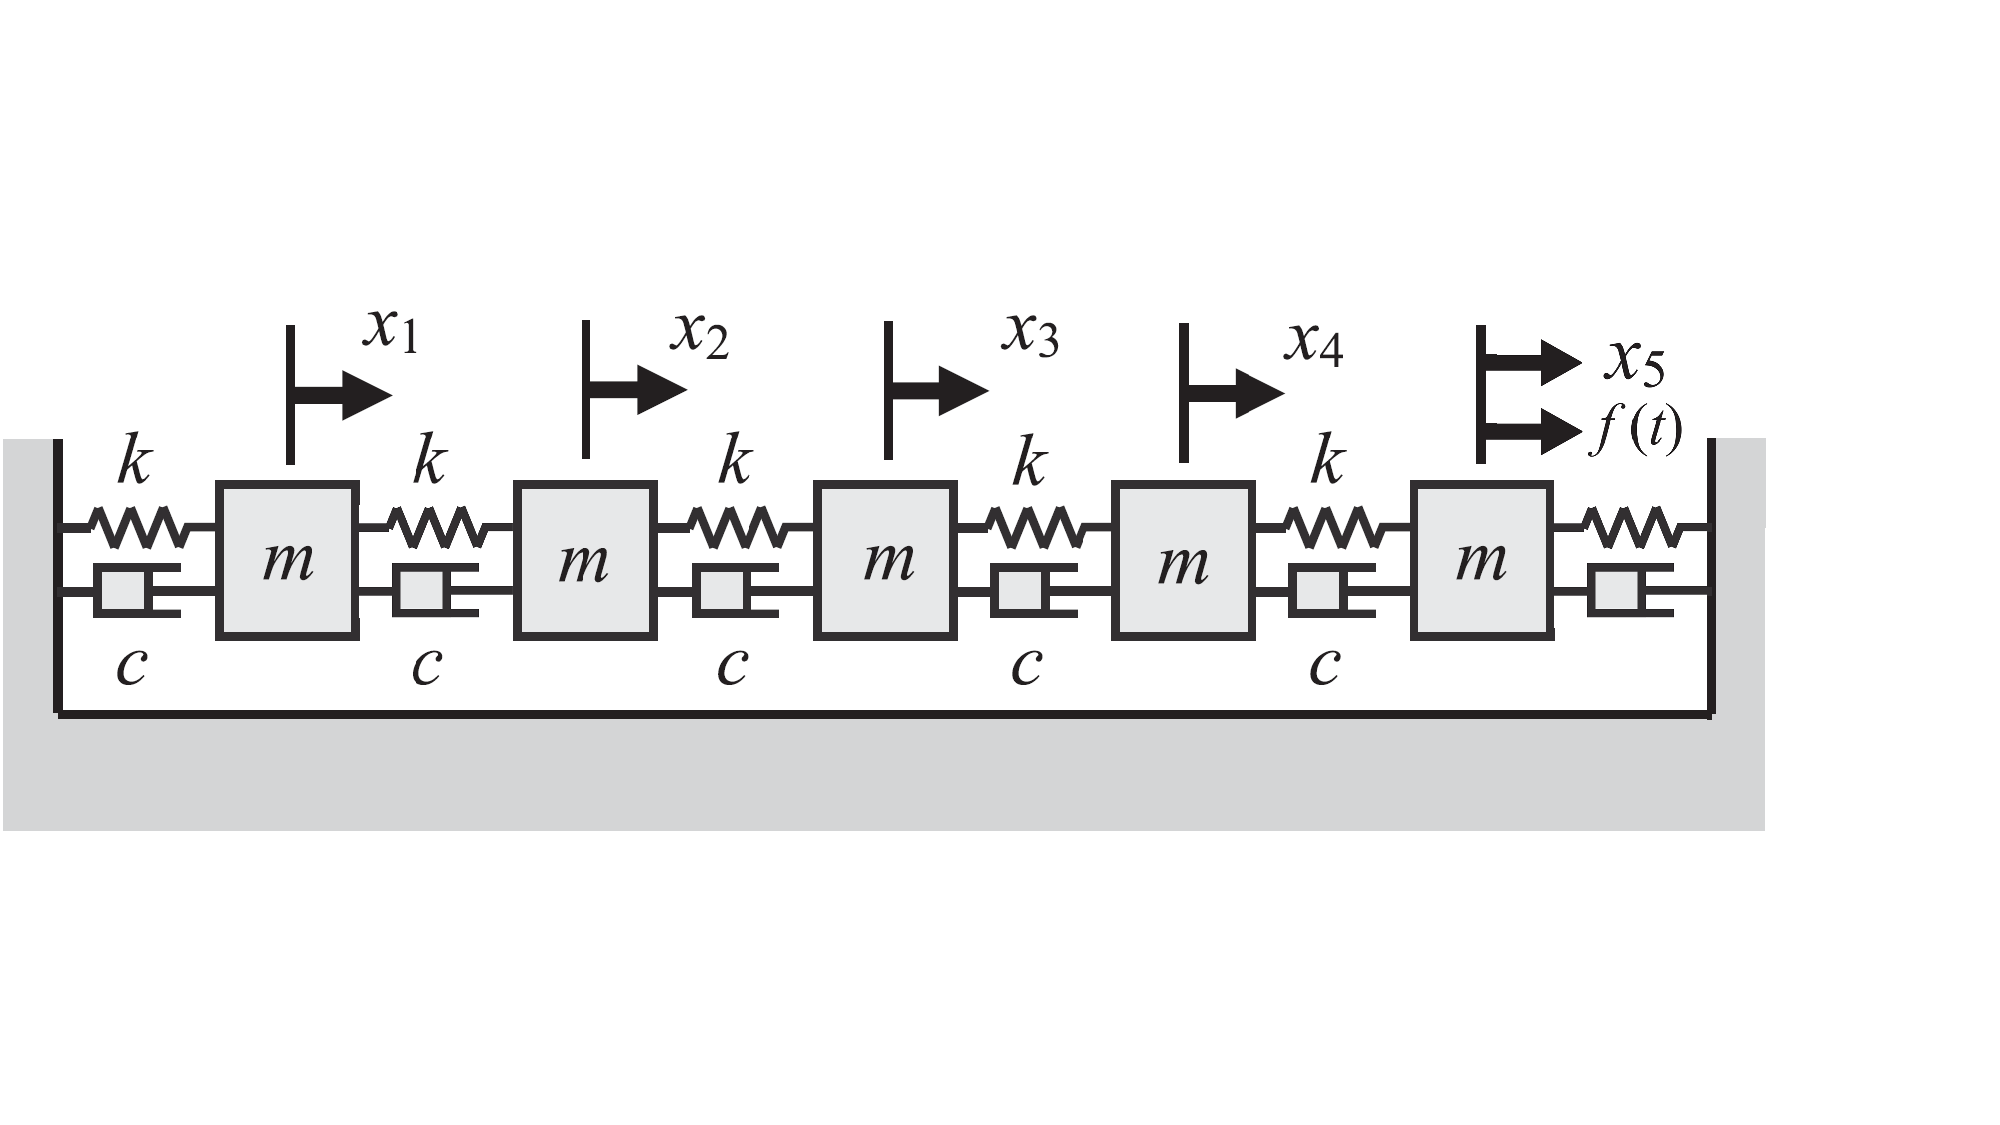
\includegraphics[width=0.5\textwidth]{Five_degree of_freedom_system.pdf}
  \end{figure}

  \begin{itemize}
    \item  The damping matrix, \( C \), is proportionally related to the stiffness matrix, defined as \( C = (c/k)K \), with \( c \) being the damping coefficient.
    \item  For the purposes of numerical example generation, the parameters are set to \( m = 1 \), \( c = 0.06 \), and \( k = 1 \). 
  \end{itemize}
  

    The stiffness matrix \( K \) is given by:
    \[
      K = \begin{bmatrix}
      2k & -k & 0 & 0 & 0 \\
      -k & 2k & -k & 0 & 0 \\
      0 & -k & 2k & -k & 0 \\
      0 & 0 & -k & 2k & -k \\
      0 & 0 & 0 & -k & 2k
      \end{bmatrix}
      \]
\end{frame}



\begin{frame}{Numerical Example: MDOF systems}
\begin{itemize}
  \item An initial excitation is applied to the fifth node.
  \item The Newmark-beta numerical method is implemented.
  \item The process continues with a time step of 0.005 seconds, covering an extensive duration of 1000 seconds.
\end{itemize}

  \begin{figure}[!ht]
    \centering
    \begin{subfigure}{0.45\textwidth}
        \centering
        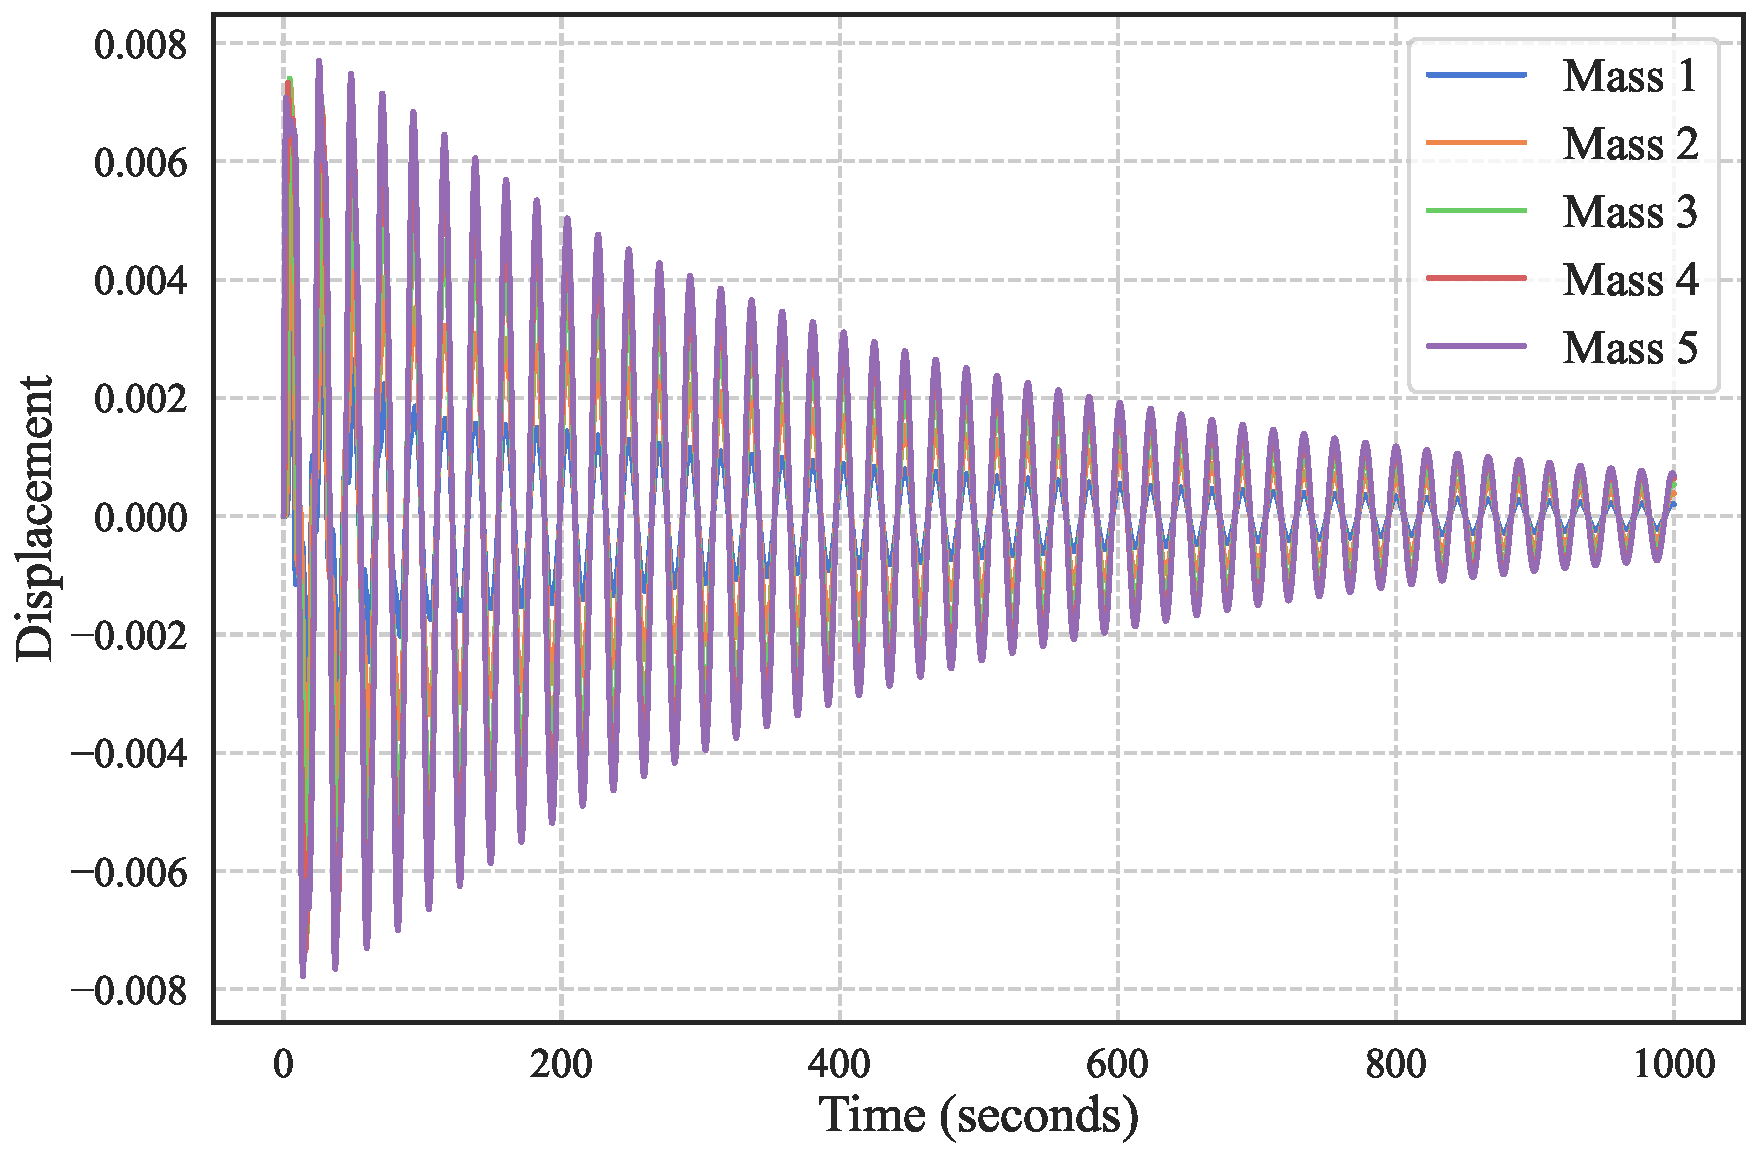
\includegraphics[width=\textwidth]{displacements_visualization.pdf}
        \caption{Time response of displacements}
    \end{subfigure}
    \hspace{2em}% Space between figures
    \begin{subfigure}{0.45\textwidth}
        \centering
        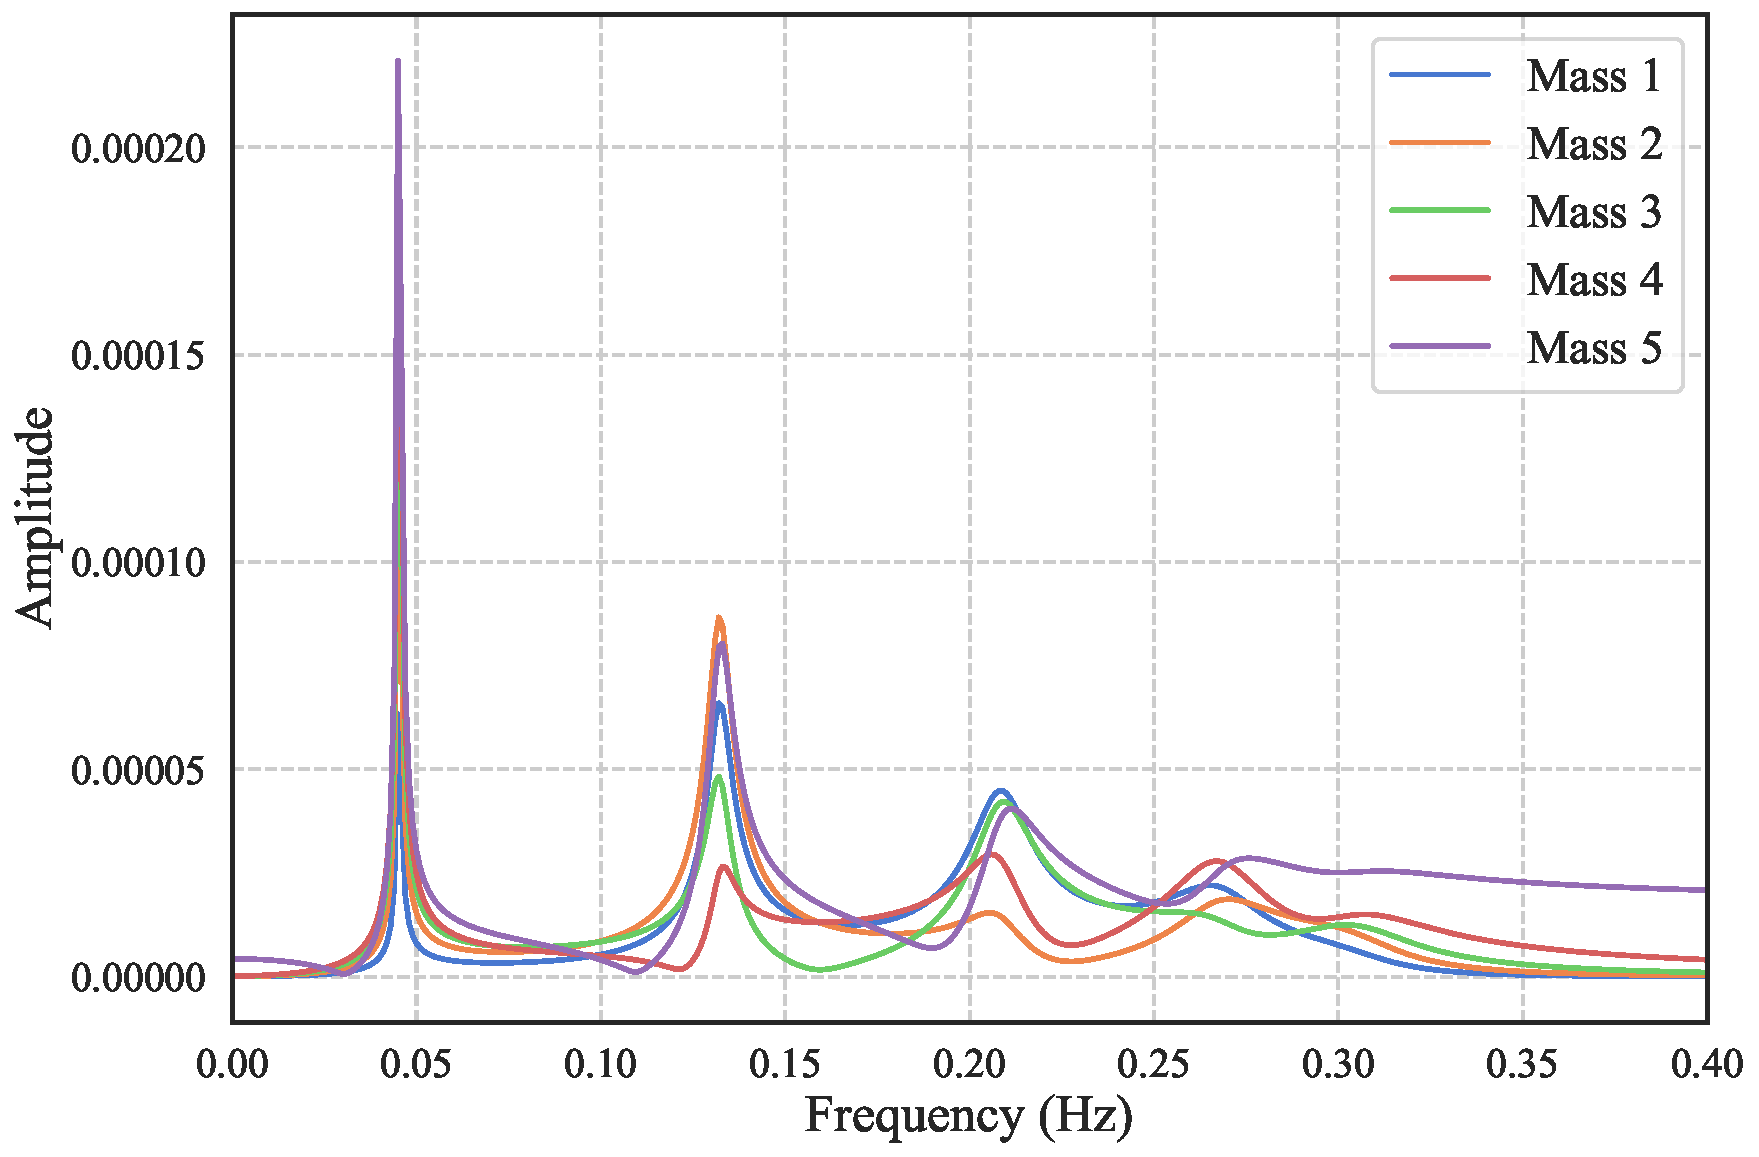
\includegraphics[width=\textwidth]{frequency_visualization.pdf}
        \caption{Frequency response of accelerations}
    \end{subfigure}
    \caption{Time response of Five degrees of freedom system}
    \label{fig:12}%\ref{fig:12}
  \end{figure}
\end{frame}


\begin{frame}{Numerical Example: MDOF systems}

  The analysis incorporates white noise proportional to signal amplitude, with each data point increased by noise amounting to 10\% of its amplitude.

  \begin{figure}[!ht]
    \centering
    \begin{subfigure}{0.31\textwidth}
        \centering
        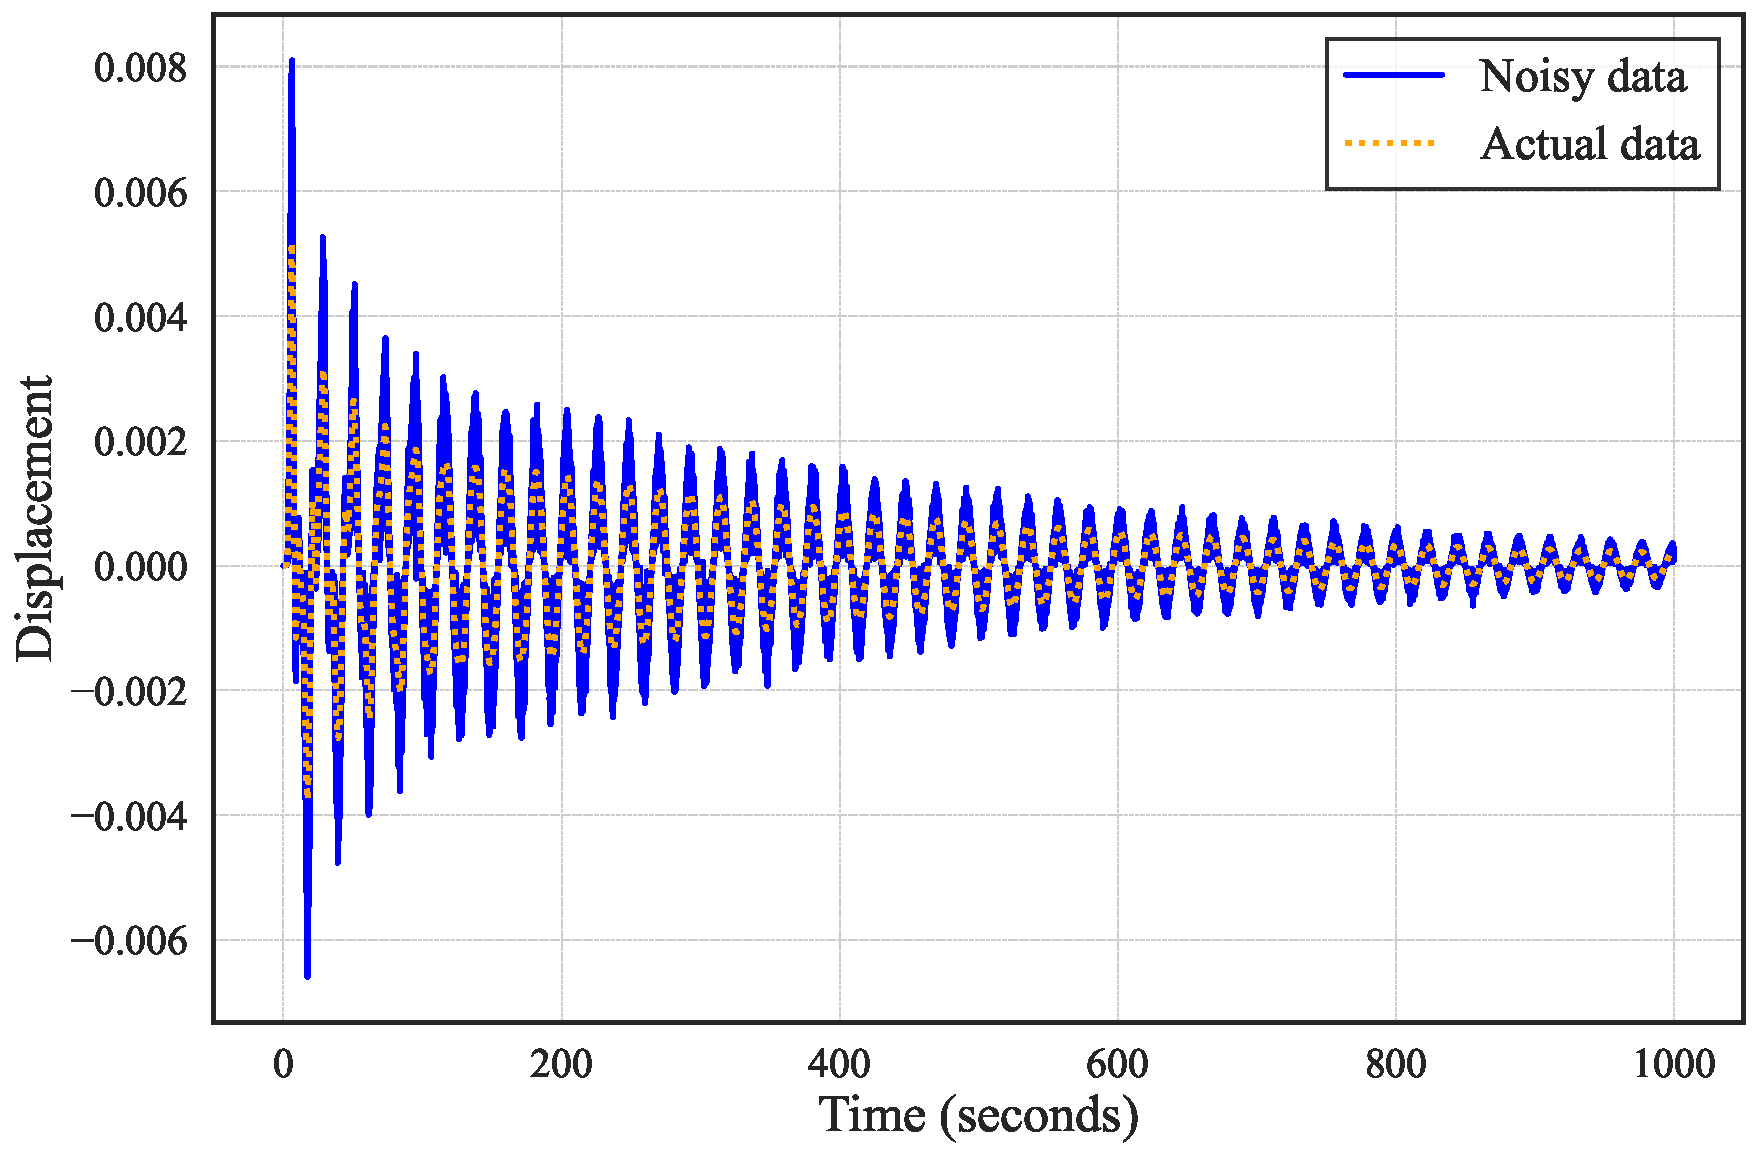
\includegraphics[width=\textwidth]{noised_displacement_vs_actual_mass_1.pdf}
        \caption{ $x_1(t)$ Displacement}
    \end{subfigure}
    \hspace{0.5em}% Space between figures
    \begin{subfigure}{0.31\textwidth}
        \centering
        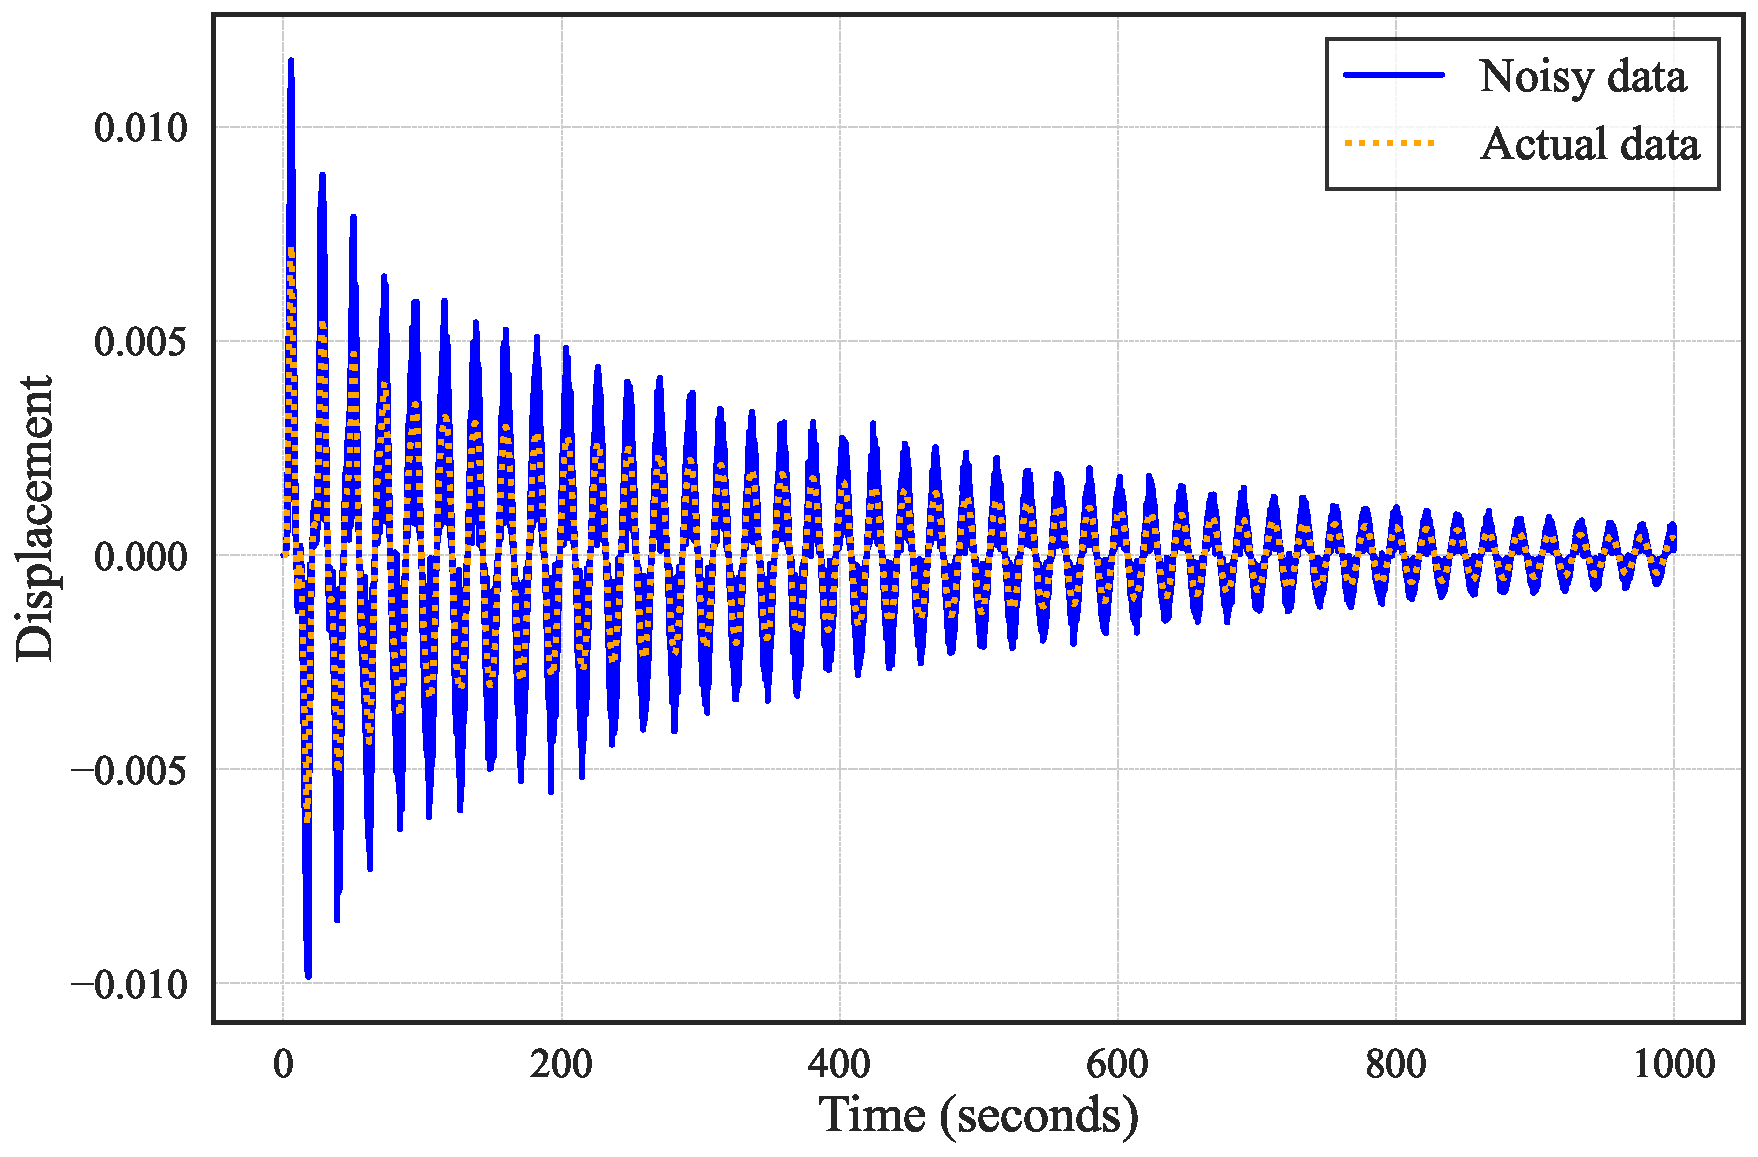
\includegraphics[width=\textwidth]{noised_displacement_vs_actual_mass_2.pdf}
        \caption{$x_2(t)$ Displacement}
      \end{subfigure}
      \hspace{0.5em}% Space between figures
      \begin{subfigure}{0.31\textwidth}
          \centering
          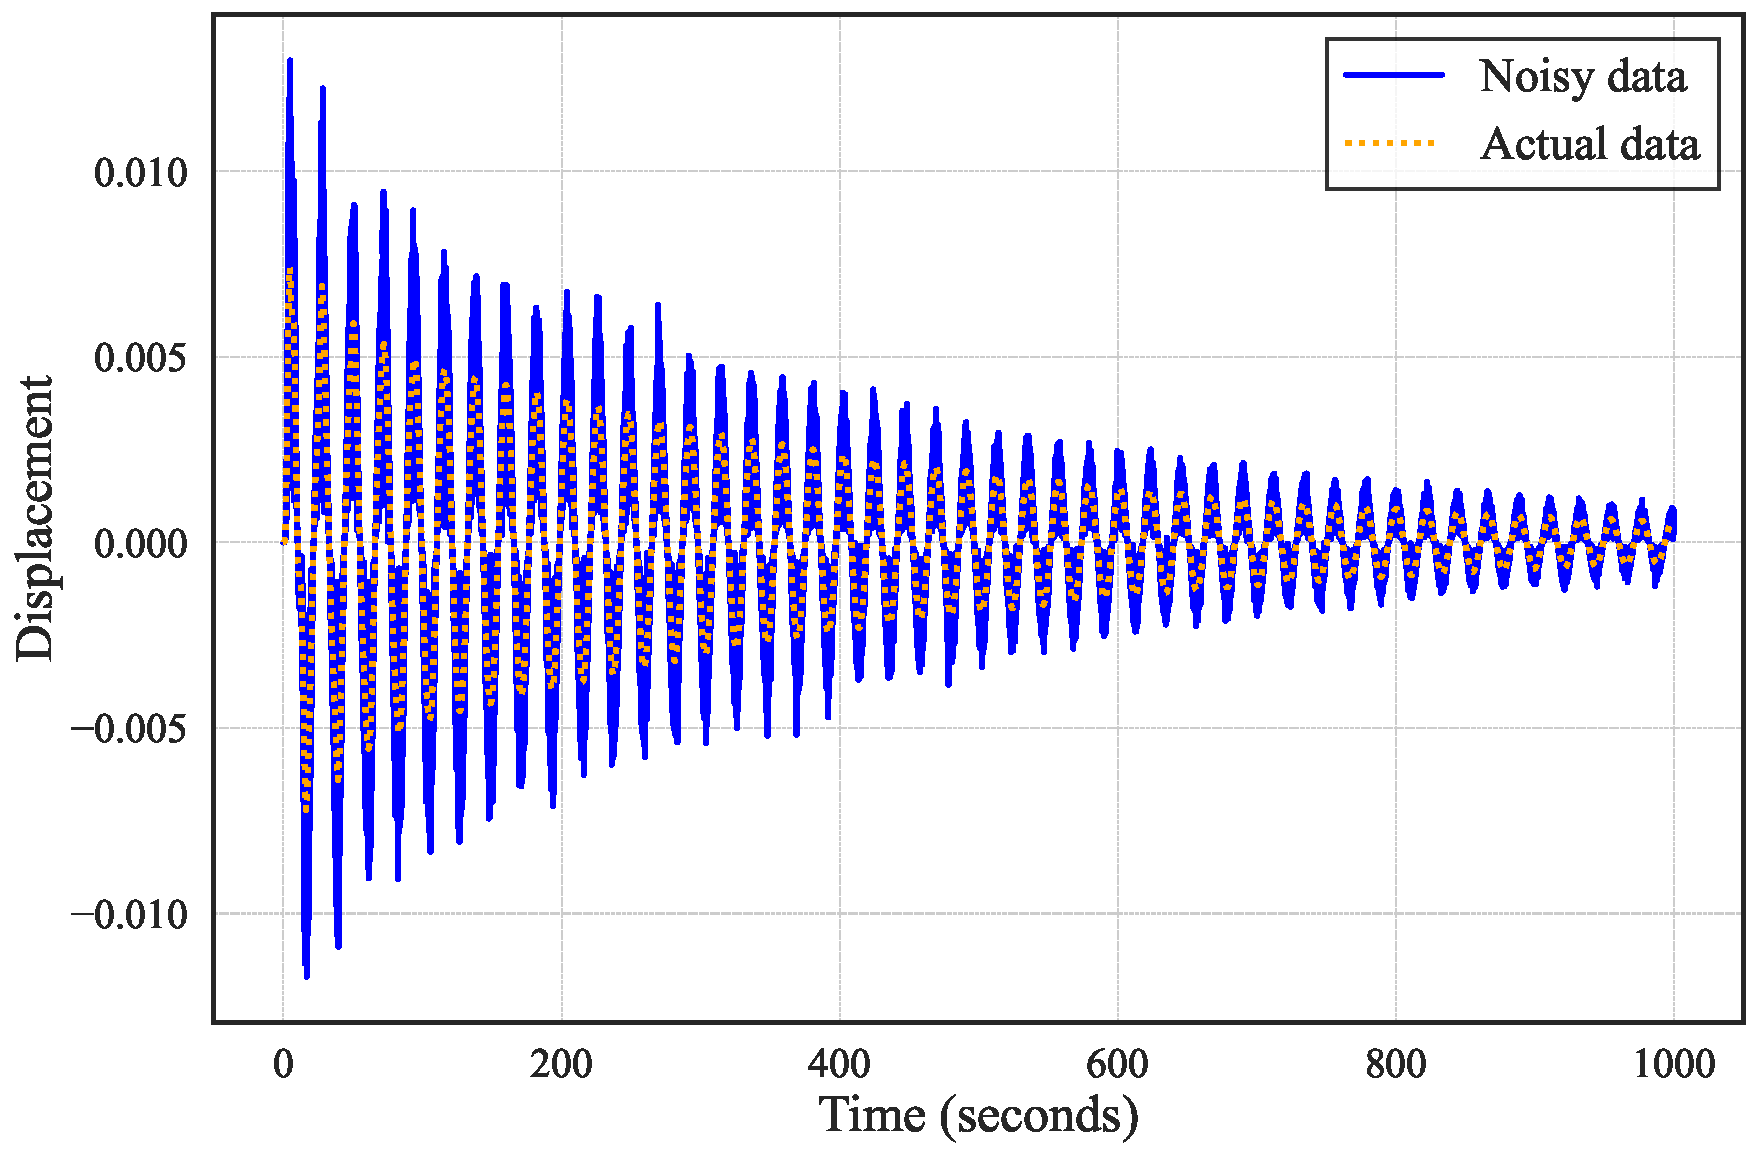
\includegraphics[width=\textwidth]{noised_displacement_vs_actual_mass_3.pdf}
          \caption{$x_3(t)$ Displacement}
    \end{subfigure}
  
    \vspace{0.5em}% Space between the two rows of figures
    \begin{subfigure}{0.31\textwidth}
        \centering
        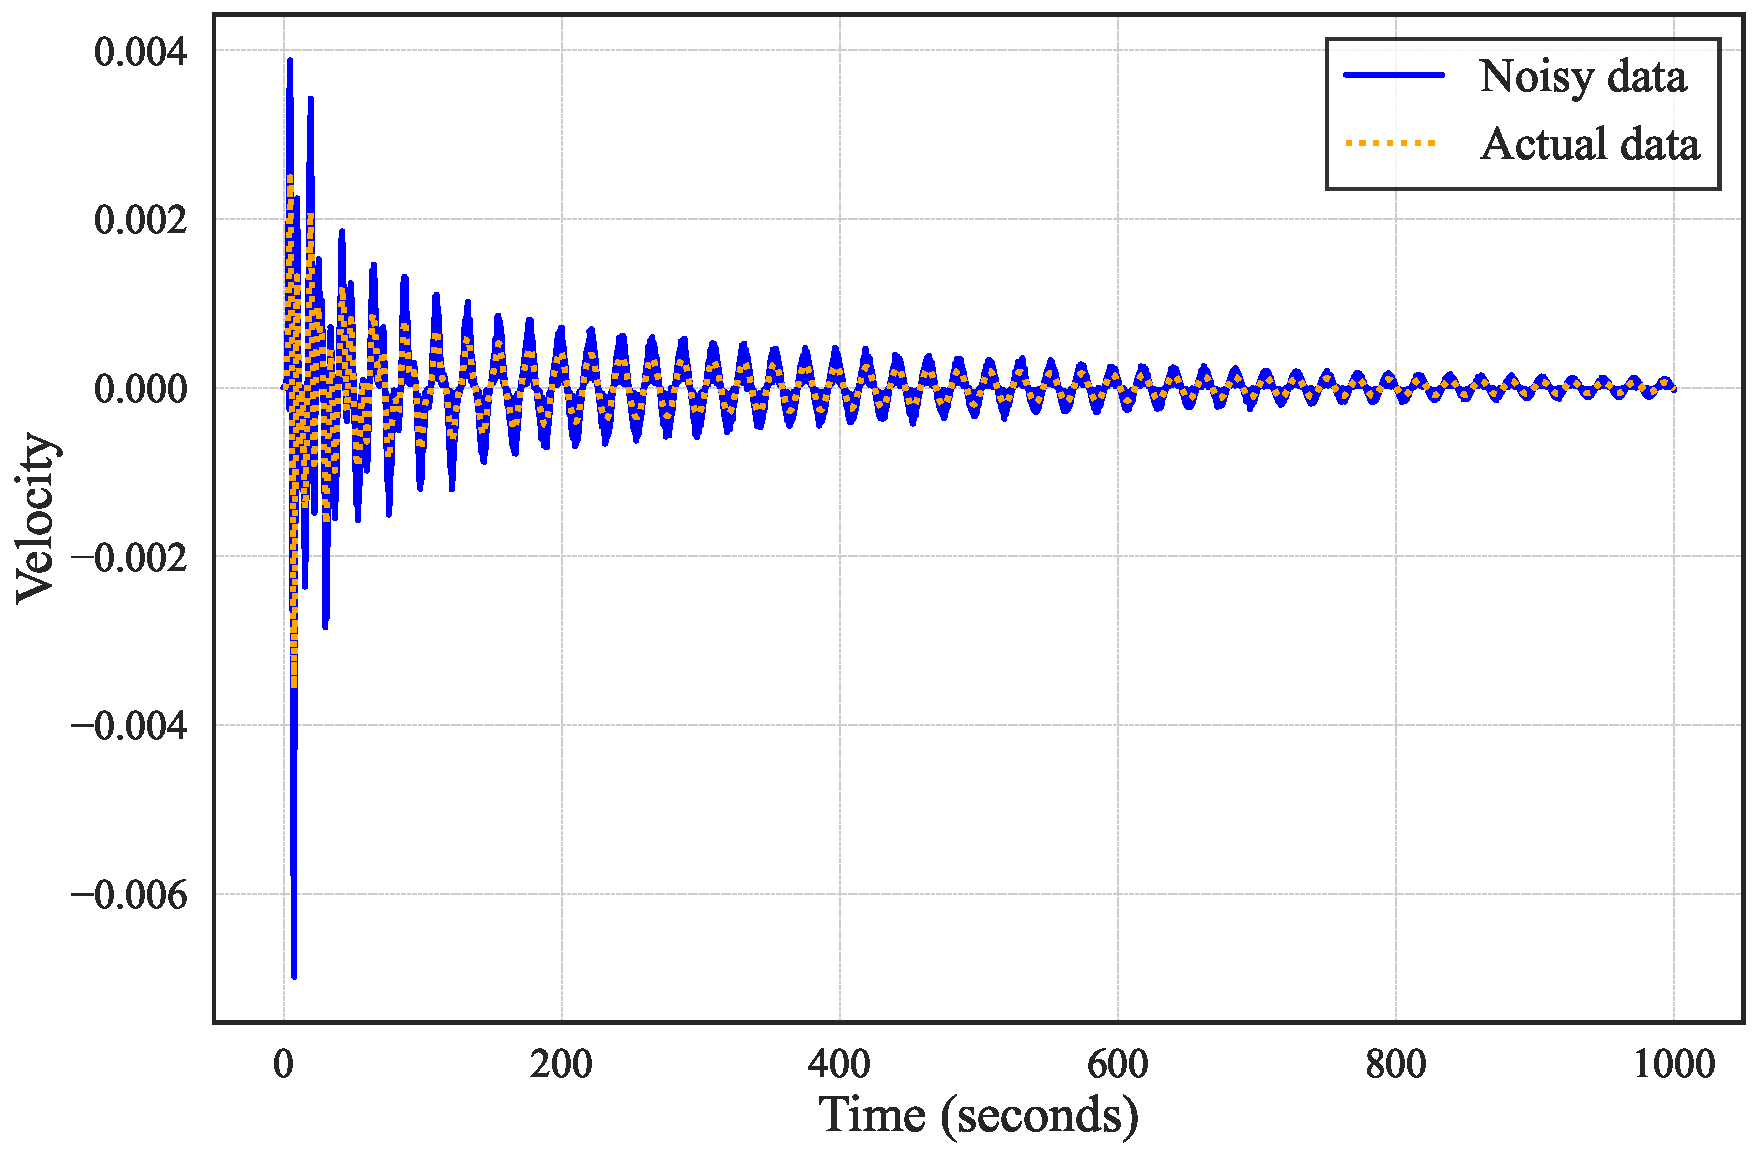
\includegraphics[width=\textwidth]{noised_Velocity_vs_actual_mass_1.pdf}
        \caption{ $x_1(t)$ Velocity}
    \end{subfigure}
    \hspace{0.5em}% Space between figures
    \begin{subfigure}{0.31\textwidth}
        \centering
        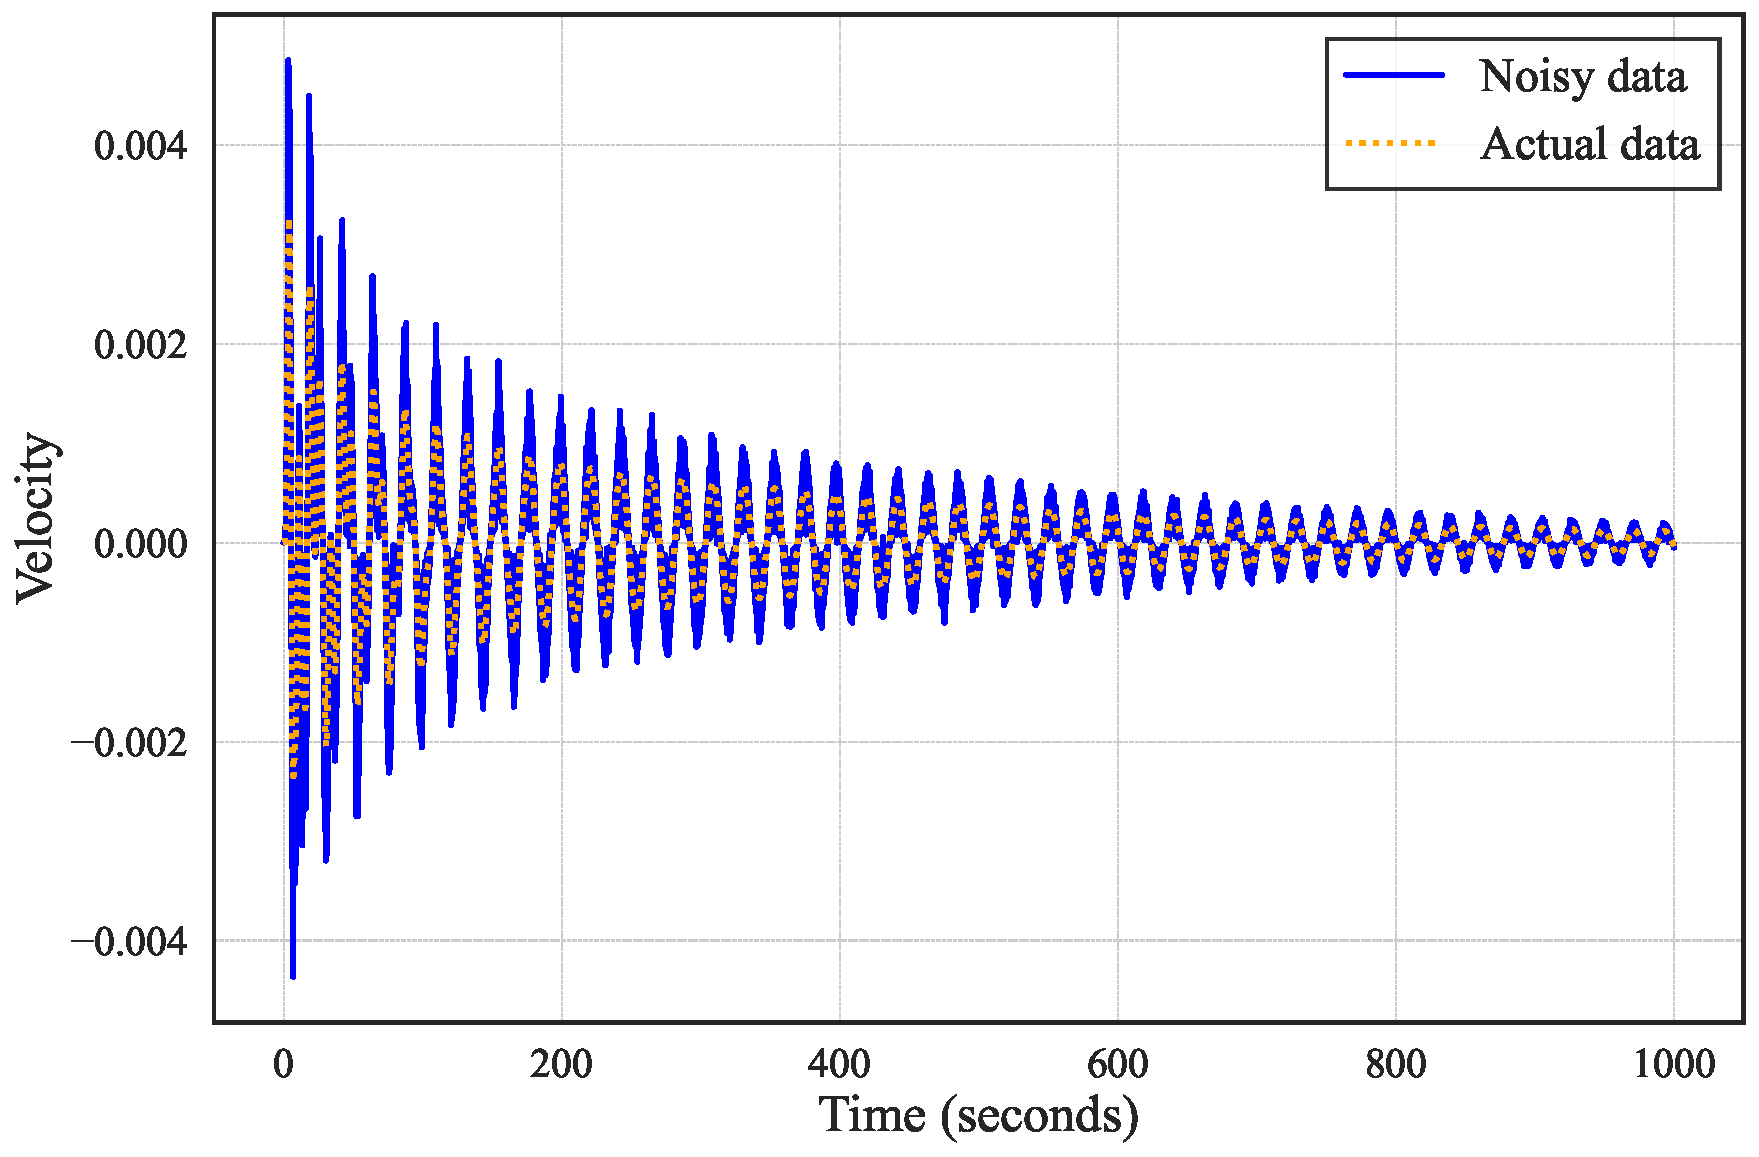
\includegraphics[width=\textwidth]{noised_Velocity_vs_actual_mass_2.pdf}
        \caption{$x_2(t)$ Velocity}
    \end{subfigure}
    \hspace{0.5em}% Space between figures
    \begin{subfigure}{0.31\textwidth}
      \centering
      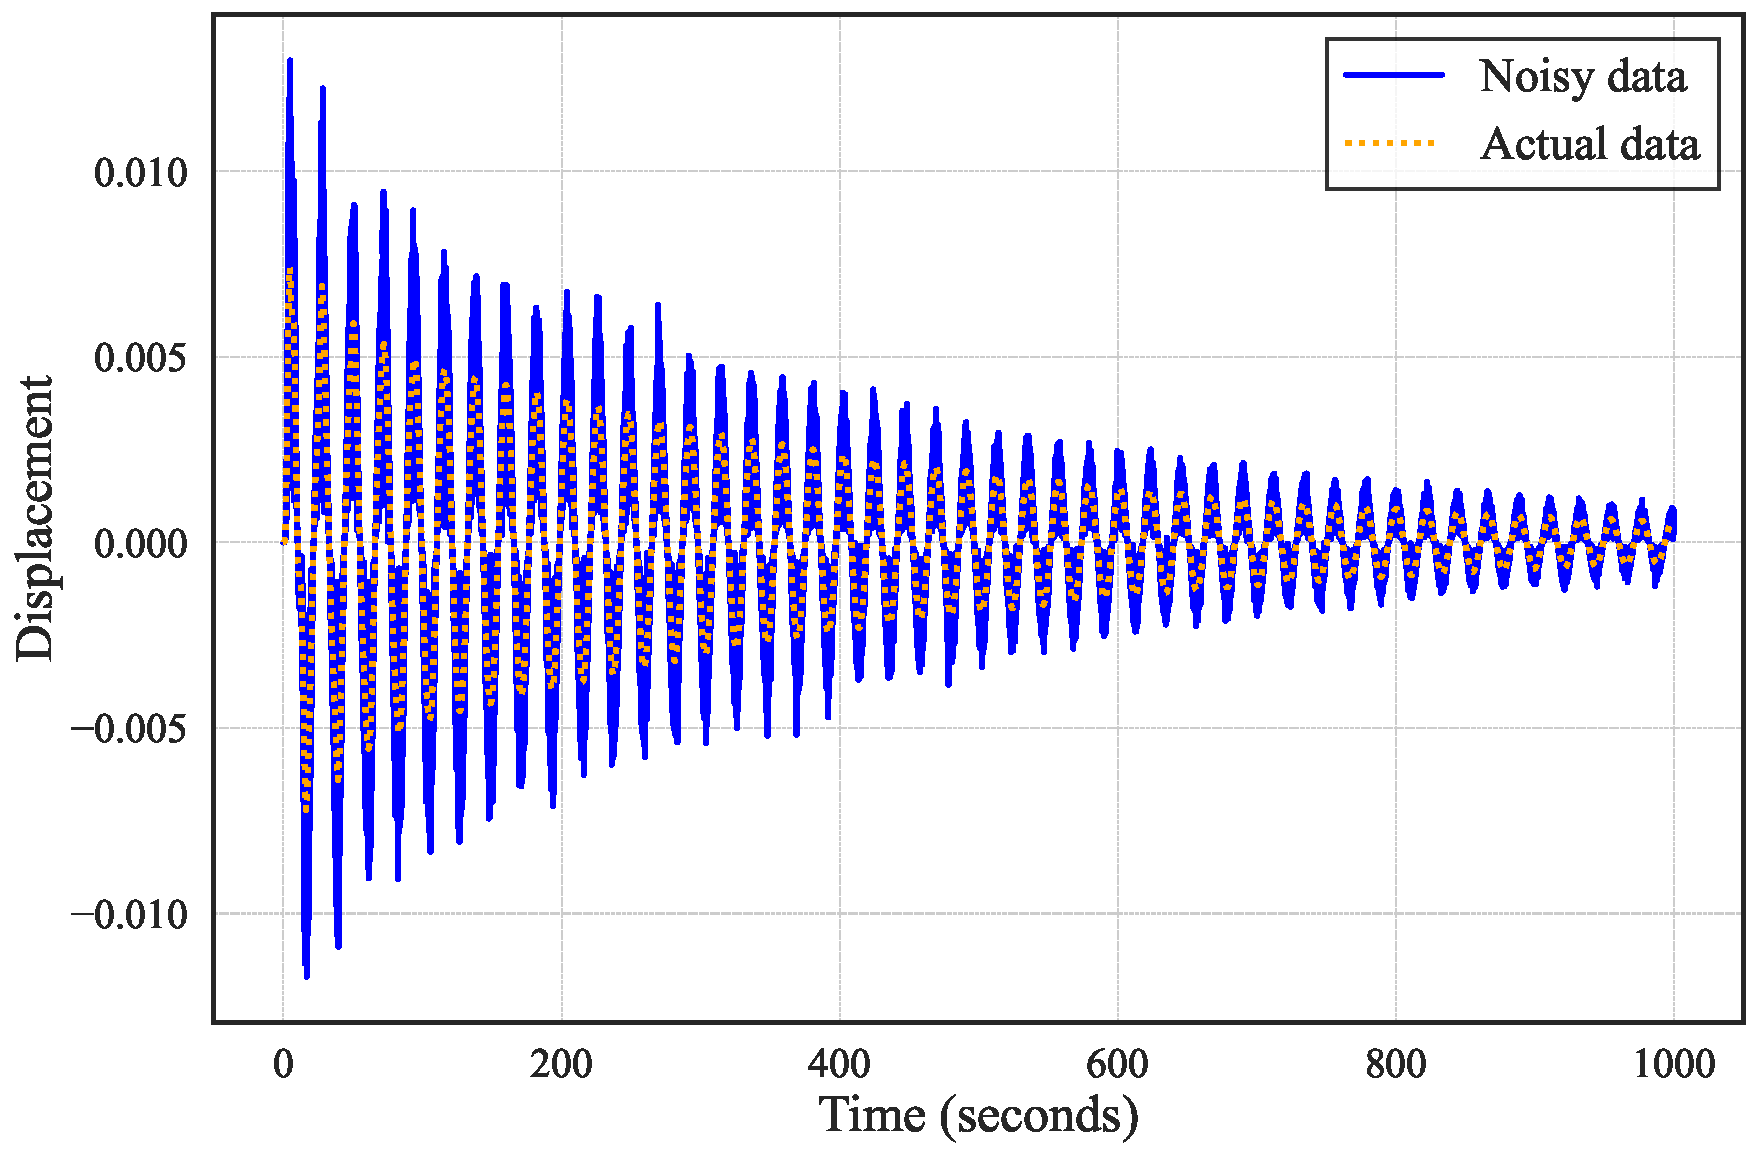
\includegraphics[width=\textwidth]{noised_displacement_vs_actual_mass_3.pdf}
      \caption{$x_3(t)$ Velocity}
  \end{subfigure}
    \label{fig:13}%\ref{fig:13}
  \end{figure}
\end{frame}


\begin{frame}{Normalized Mean Squared Error }
  The Normalized Mean Squared Error (NMSE) is a metric used to evaluate the accuracy of a predictive model:
  \[
  \text{NMSE} = \frac{\sum_{i=1}^{N} (y_i - \hat{y}_i)^2}{\sum_{i=1}^{N} (y_i - \bar{y})^2}
  \]
  where \( y_i \) is the \(i\)-th true value, \( \hat{y}_i \) is the \(i\)-th predicted value, \( \bar{y} \) is the mean of the true values calculated as \( \bar{y} = \frac{1}{N} \sum_{i=1}^{N} y_i \), and \( N \) is the number of samples.
  \begin{itemize}
    \item  \textbf{NMSE ≈ 0}: Indicates nearly perfect model predictions with minimal error. The predicted values are very close to the true values.
    \item \textbf{0 < NMSE < 0.1:} Indicates very accurate model predictions with small errors. The predicted values are very close to the true values. 
    Such models are considered highly accurate.
    \item \textbf{NMSE ≥ 1:} Indicates very high prediction errors. The predicted values may be worse than using the mean value as the prediction. Such models are generally considered invalid and require major improvements.
  \end{itemize}
\end{frame}




\subsection{Hamilton's Principle}

\begin{frame}{The form of the Equations of Motion}
  \textbf{Differential and Integral Forms:}
  
  \begin{itemize}
    \item The \textcolor{red}{differential} form refers to describing the state and changes of the system at every moment using differential equations. This form focuses on the specific behavior of the system at each instant.
    \item The \textcolor{red}{integral} form refers to describing the state and changes of the system over a longer period using integral equations. This form emphasizes the overall behavior of the system over a certain period.
  \end{itemize}
  
  \textbf{Non-Variational and Variational Forms:}
  \begin{itemize}
    \item The \textcolor{red}{non-variational} form refers to describing the motion of the system using physical quantities such as force, mass, and acceleration, focusing on the general laws of all actual movements.
    \item The \textcolor{red}{variational} form refers to describing the system's motion through variational principles. 
    The variational principle considers that, among all possible motion paths, the actual motion path is the one that extremizes a certain action.
  \end{itemize}
  \end{frame}



  \begin{frame}{Hamilton's Principle}
Hamilton's variational statement of Dynamics:
\[
\int_{t_1}^{t_2} \delta [T(t) - V(t)] \, dt + \int_{t_1}^{t_2} \delta W_{nc}(t) \, dt = 0
\]
where \(T(t)\): The kinetic energy of the system at time \(t\), \(V(t)\): The potential energy of the system at time \(t\), and \(W_{nc}(t)\): The work done by nonconservative forces at time \(t\).

\begin{itemize}
  \item Hamilton's Principle can be interpreted as stating that the actual path taken by the system between times \(t_1\) and \(t_2\) 
  is such that the integral of the variation of the difference between kinetic and potential energies plus the integral of the variation of 
  the work done by nonconservative forces is zero. 
  \item The application of Hamilton's Principle leads directly to the equations of motion for any given system.
\end{itemize}
\end{frame}

\begin{frame}{Hamilton's Principle}
  When applied to statics problems, the kinetic-energy term \( T \) vanishes, and the remaining terms in the integrands are invariant with time. Thus, the equation reduces to:
  \[
  \delta (V - W_{nc}) = 0
  \]
  which is the well-known \textbf{principle of minimum potential energy}. The equations of motion for an \(N\)-Degrees of Freedom system can be derived directly from Hamilton's Principle by simply assuming:
   \begin{align*}
    T &= T(q_1, q_2, \cdots, q_N, \dot{q}_1, \dot{q}_2, \cdots, \dot{q}_N)\\
    V &= V(q_1, q_2, \cdots, q_N) \\
    \delta W_{nc} &= Q_1 \delta q_1 + Q_2 \delta q_2 + \cdots + Q_N \delta q_N 
  \end{align*}
  where \(q_1, q_2, \cdots, q_N\) represent a set of generalized coordinates, and the coefficients \(Q_1, Q_2, \cdots, Q_N\) are the generalized forcing functions corresponding to the coordinates \(q_1, q_2, \cdots, q_N\), respectively.
\end{frame}

\begin{frame}{Lagrange's Equations}
  By substituting the aforementioned expressions into Hamilton's variational statement of dynamics, Lagrange's equations of motion are given by:
  \[
  \frac{d}{dt} \left( \frac{\partial T}{\partial \dot{q}_i} \right) - \frac{\partial T}{\partial q_i} + \frac{\partial V}{\partial q_i} = Q_i
  \]
  Consider the \textbf{double pendulum under free vibration conditions}\cite{1977Dynamics}. The equations of motion can be derived using Lagrange's Equations as follows:
  \begin{figure}[htpb]
    \centering
    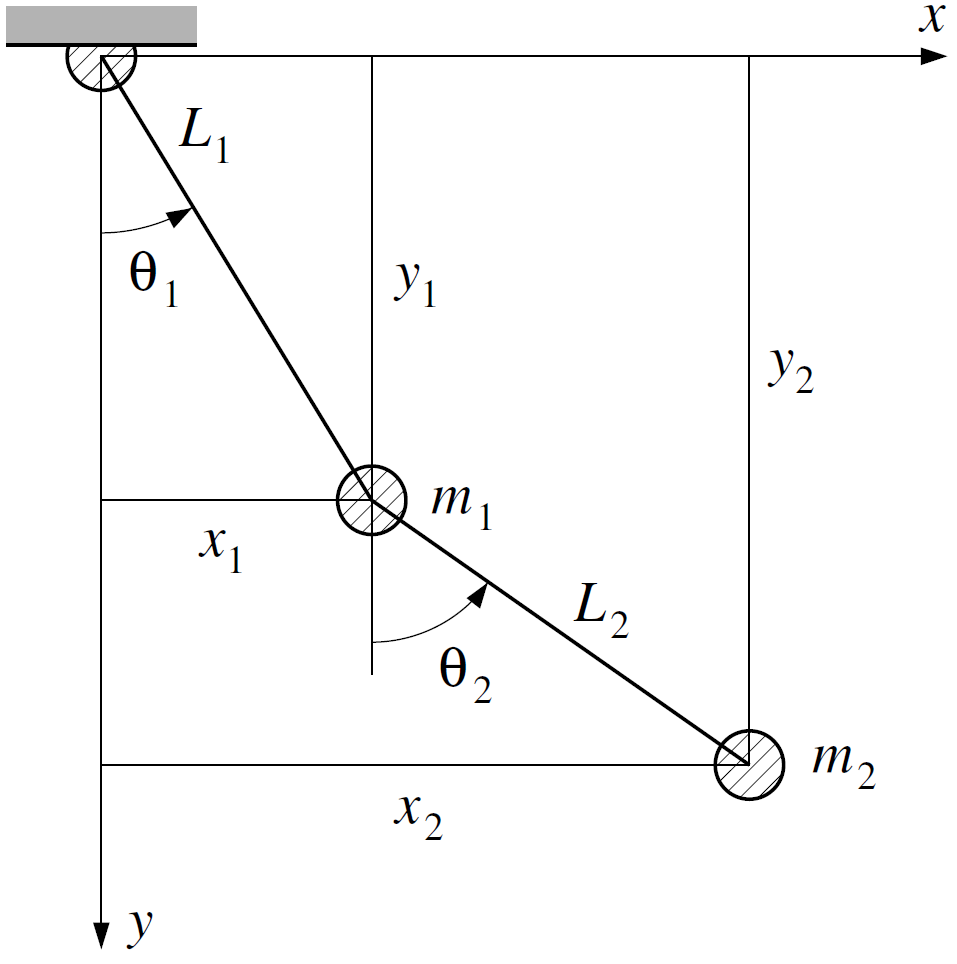
\includegraphics[width=0.33\textwidth]{double_.png}
  \end{figure}
\end{frame}




\begin{frame}{Lagrange's Equations}
  The kinetic energy and potential energy of the double pendulum can be expressed in terms of the set of generalized coordinates \( q_1 \equiv \theta_1 \) and \( q_2 \equiv \theta_2 \) as follows:
  \begin{align*}
      T &= \frac{1}{2} m_1 L_1^2 \dot{q}_1^2 + \frac{1}{2} m_2 \left[ L_1^2 \dot{q}_1^2 + L_2^2 \dot{q}_2^2 + 2 L_1 L_2 \dot{q}_1 \dot{q}_2 \cos(q_2 - q_1) \right] \\
      V &= (m_1 + m_2) g L_1 (1 - \cos q_1) + m_2 g L_2 (1 - \cos q_2)
  \end{align*}
  
  Since there are no nonconservative forces acting on this system, substituting into Lagrange's Equation yields:
  \begin{align*}
    (m_1 + m_2) L_1^2 \ddot{q}_1 + m_2 L_1 L_2 \ddot{q}_2 \cos (q_2 - q_1) &- m_2 L_1 L_2 \dot{q}_2^2 \sin (q_2 - q_1) \notag \\
    &+ (m_1 + m_2) g L_1 \sin q_1 = 0 \\
    m_2 L_2^2 \ddot{q}_2 + m_2 L_1 L_2 \ddot{q}_1 \cos (q_2 - q_1) &+ m_2 L_1 L_2 \dot{q}_1^2 \sin (q_2 - q_1) \notag \\
    &+ m_2 g L_2 \sin q_2 = 0
  \end{align*}
  \end{frame}
  

  \begin{frame}{The General Equations of Motion for Linear Systems}

    As long as the energy and work terms can be expressed in terms of the generalized coordinates, and of their time derivatives and variations, Lagrange's equations are valid, regardless of whether the system is linear or nonlinear.

    \vspace{0.5em}

    The kinetic and potential energies of linear engineering systems subjected to small-amplitude oscillations can be expressed in the quadratic forms:
    \[
    T = \frac{1}{2} \sum_{j=1}^{N} \sum_{i=1}^{N} m_{ij} \dot{q}_i \dot{q}_j = \frac{1}{2} \dot{\mathbf{q}}^T \mathbf{M} \dot{\mathbf{q}}
    \]
    \[
    V = \frac{1}{2} \sum_{j=1}^{N} \sum_{i=1}^{N} k_{ij} q_i q_j = \frac{1}{2} \mathbf{q}^T \mathbf{K} \mathbf{q}
    \]
    where \(N\) is the number of degrees of freedom in the system.
  \end{frame}



\begin{frame}{The General Equations of Motion for Linear Systems}
  For such systems, the second term of Lagrange's equations, namely, \(\partial T / \partial q_i\) (\(i = 1, 2, \cdots, N\)), equals zero, which reduces Lagrange's equations to the form:
  \[
  \frac{\partial}{\partial t} \left( \frac{\partial T}{\partial \dot{q}_i} \right) + \frac{\partial V}{\partial q_i} = Q_i \quad i = 1, 2, \cdots, N 
  \]
  Lagrange's equations of motion, when placed in matrix form, become:
  \[
  \mathbf{M} \ddot{\mathbf{q}} + \mathbf{K} \mathbf{q} = \mathbf{Q}
  \]
  All nonconservative forces, including damping forces, are contained here in the generalized forcing functions \(Q_1, Q_2, \cdots, Q_N\). It is evident that
  \[
  Q_i = p_i - \sum_{j=1}^{N} c_{ij} \dot{q}_j 
  \]
  Substituting into Lagrange's equations gives the governing equations of motion in matrix form:
  \[
  \mathbf{M} \ddot{\mathbf{q}} + \mathbf{C} \dot{\mathbf{q}} + \mathbf{K} \mathbf{q} = \mathbf{p} 
  \]

\end{frame}



% Third Section: Conclusion
\section{Conclusion}

% Display table of contents at the beginning of each section
\frame{\frametitle{Outline}\tableofcontents[currentsection]}
\subsection{Conclusion}
\begin{frame}{Conclusion}
  \begin{itemize}
    \item Summarize your main points.
    \item Provide conclusions and future work.
  \end{itemize}
\end{frame}

\subsection{Alert Information}
\begin{frame}
\frametitle{Alert Information}
\begin{alertblock}{Alert Information}
  \begin{itemize}
    \item This document is a Beamer template for HITsz students and faculty, created on July 1, 2024.
    \item Users are encouraged to make further revisions and improvements to this template for educational purposes.
    \item This template is not intended for commercial use. If you wish to distribute it, please contact the email below in advance and attribute the source appropriately.
    \item Licensed under the MIT License. See the LICENSE file for more details.
    \item This template is provided "as is", without warranty of any kind, express or implied.
  \end{itemize}
\end{alertblock}
\end{frame}



% Final Section: Thank You
\section*{}
\begin{frame}{}
  \begin{center}
      \begin{minipage}{1\textwidth}
          \setbeamercolor{mybox}{fg=white, bg=black!50!blue}
          \begin{beamercolorbox}[wd=0.8\textwidth, rounded=true, shadow=true]{mybox}
              \centering \LARGE \textbf{Thank you for your valuable time.}
          \end{beamercolorbox}
      \end{minipage}
      \\[20pt]
      \LARGE Please feel free to contact us:
      \\[10pt]
      23B954005@stu.hit.edu.cn
      \\[20pt]
      
\includegraphics[width=0.5\linewidth]{hitsz.pdf}
  \end{center}
\end{frame}

\bibliographystyle{plain} 
\bibliography{references}

% End of document
\end{document}
